In this chapter, my aim is to introduce the reader to the concept of multiple criteria decision making in the
context of multi-objective optimization. Motivation, and an informal introduction to the 
central concepts, will be given in \ref{mcdmintro}. The following sections will dive deeper into the concepts, with
multi-objective optimization being presented in \ref{multiopt}. Methods for solving multi-objective optimization problems will be
presented in \ref{mcdmsolve}. In section \ref{mcdmdm} I will define what is meant by a decision maker, and how their preference
can be modelled. This chapter will conclude with section \ref{mcdminter} where I will explain what interactive methods are,
 why they are important, and I will reference methods in literature as examples of interactive methods.
 
The concepts presented in this chapter are fundamental to optimization. Various works can be found, such as \cite{Miettinen1998} and
\cite{yoshikazusawaragi1985}, to which I encourage the reader to refer to, if a more in-depth analysis of the presented concepts in this
chapter is desirable. My goal is to present a solid enough overview of the concepts in optimization that are relevant to this thesis.

\section{Introduction}
\label{mcdmintro}
A CEO of a multi-billion corporation has to decide what course to take, in terms of managing her business, in the
coming financial year to maximize the profit
of her corporation, and keeping the stake holders happy. A student is at his wit's end: Should he take a quickie
loan\footnote{A small loan that is quick and easy to get, but has a very high interest rate.}
to afford proper food, or should he swallow
his pride and fare with cup noodles for the rest of the month. A recruiter for a local supermarket has a couple of possible
candidates available for an open cashier job position: Who should the recruiter choose? The CEO, student, and recruiter, are
all very different people in very different situations, but what connects them, is that they are all trying to make
some decision.

In the previous scenarios, the CEO, student, and recruiter, are all in the position of a decision maker: They have
to make a decision based on the information available to them. The student, for example, has to decide whether to
take a small loan now to afford proper food, but with the increased cost of interests to be paid, or not to take a
loan, saving money, but having to cope with miserable food. It can be said, that the student has two objectives:
Minimizing his financial losses, and maximizing the quality of food. The student has also realized, to his knowledge or not,
that he cannot have gourmet food without paying a high cost, and he cannot pay pennies and expect a filet mignon. There is a
a trade-off between quality of food, and the money in his bank account; gaining in quality of food will lead to a loss
of capital, and trying to save money results in worse quality of food. It doesn't take much imagination to
imagine the CEO and the recruiter having to make similar trade-offs when deciding what to do.

This kind of decision making, where multiple criteria are conflicting, is at the heart multiple criteria decision making,
or MCDM in short. This thesis has a special focus on modelling the decision maker's behavior in a MCDM context. The concept
of preference also arises: Given a set of options, where no option can be traded to an other option without a loss in
some criteria, what option should a decision maker choose, and why did they choose that option? An underlying preference
guides the decision maker, and understanding this preference, can give insight into the logic of the decision maker,
which in turn, helps understand why the decision maker has made the decision he/she made.

\section{Optimization}
\label{multiopt}
In this section, my goal is to define what is meant by a multi-objective optimization problem. I will start by defining
a single-objective optimization problem in \ref{singleobj}, from which I will generalize the concepts to the concept of a multi-objective
optimization problem in \ref{multiobj}. Lastly, I will define concepts unique to multi-objective optimization problems in \ref{multiconcepts}.

The concepts presented in this chapter are fundamental to optimization. Various works can be found, such as \cite{Miettinen1998} and
\cite{yoshikazusawaragi1985}, which the reader is encourages to refer to, if a more in-depth analysis of the presented concepts in this
chapter is desired.

\subsection{Single-objective optimization}
\label{singleobj}
Before a multi-objective optimization problem can be formally defined, a general case of a single-objective optimization problem is
formulated. Based on this formulation, the formal definition of a multi-objective optimization problem, and related concepts, is
given later in this section.

In a single-objective optimization problem, an objective is usually defined as a scalar valued function of
one or multiple
independent variables. Both the function
and variables are real or integer valued. Formally, a single objective can be defined as

\begin{equation}
    \label{eq:objective}
    f: \mathbb{R}^n \to \mathbb{R},
\end{equation}

where $n$ denotes the number of dimensions in the domain of the objective function $f$, or in
other words, the number of variables the function is defined for.

The input variables, often called decision variables, for an objective function defined in \eqref{eq:objective},
can be defined as a vector
of independent variables, also called a decision variable vector:

\begin{equation}
    \label{eq:variablevector}
    \mathbf{x} = \Set{x_i \mid \forall i \in \left[1, n\right]},
\end{equation}

where $x_i$ denotes the value of the $i$th attribute. In the context of a single-objective optimization problem,
the variables of an objective function are often subject to constraints defined in the problem.
These constraints can be 
inequality constraints or equality constraints defined as:

\begin{equation}
    \label{eq:inequality}
    g_k: \mathbb{R}^{n_k} \to \mathbb{R}:\; g_k(\mathbf{x}) \leq 0,\quad\text{where}\;k\in\left[1, K\right],\;\text{and}\;n_k\leq n,
\end{equation}

and

\begin{equation}
    \label{eq:equality}
    h_l: \mathbb{R}^{n_l}\to\mathbb{R}:\;h_k(\mathbf{x}) = 0,\quad\text{where}\;l\in\left[1, L\right],\;\text{and}\;n_l\leq n.
\end{equation}

In \eqref{eq:inequality} and \eqref{eq:equality}, $K$ and $L$ denote, respectively,
the total number of that particular type of constraints present in the problem. The constraints in a single-objective
optimization problem define a certain feasible space for the variables $\mathbf{x}$, which can be denoted
as the feasible set $X$ of decision variable vectors. Therefore, the feasible decision variable vectors, of a single-objective
optimization problem, can be
denoted as

\begin{equation}
    \label{eq:feasibledecisionset}
    \mathbf{x} \in X \subseteq \mathbb{R}^n.
\end{equation}

In the case of $X=\mathbb{R}^n$ in \eqref{eq:feasibledecisionset}, the underlying optimization problem is said to be
unconstrained, where as in the case of $X\subset\mathbb{R}^n$, the problem is said to be constrained.

Based on the concepts defined so far, the full definition of a single-objective optimization problem can be given as

\begin{equation}
    \label{eq:singleobjectiveproblem}
    \max_{\mathbf{x}\in X} f(\mathbf{x}),
\end{equation}

where the objective function $f$ is to be maximized, and the decision variable vector $\mathbf{x}$ must be part of the feasible decision variable
vector space $X$. The choice of whether an objective function should be maximized or minimized, is arbitrary, but usually stems from the
nature of the objective in the optimization problem; profits are to be maximized, and losses are to be minimized. If need be, a maximization
problem can be transformed into a minimization problem by multiplying the objective by $-1$. For example, \eqref{eq:singleobjectiveproblem}
is equivalent to

\begin{equation}
    \label{eq:minussingleobjectiveproblem}
    \min_{\mathbf{x}\in X} -f(\mathbf{x}).
\end{equation}

The solution to a single-objective optimization problem is therefore defined as some $\mathbf{x^*}\in X$ which satisfies 
both \eqref{eq:singleobjectiveproblem} and \eqref{eq:minussingleobjectiveproblem}. The objective functions is said to reach its'
optimal value, when given $\mathbf{x^*}$ as argument.

In some cases there might be multiple solutions
to a single-objective optimization problem, for example in the case of minimizing the objective $f: \mathbb{R}\to\mathbb{R}:\;
f(x) = |x^2 - 1|$, both solutions
$x^*_1 = 1$ and $x^*_2 = -1$ minimize the function. In this case, the solutions $x^*_1$ and $x^*_2$
are considered to be equally preferable, meaning
there is no clear benefit\footnote{If there was a clear benefit in choosing one solution over the other,
it should be formulated in either the objective function of the problem,
or as a constraint of the problem.} in choosing one solution over the other.

\subsection{Multi-objective optimization}
\label{multiobj}
Like the name of this subsection suggests, in multi-objective optimization, the number of objectives to be optimized
is greater than one. These objectives are to be optimized, either minimized or maximized, simultaneously. The objective of a multi-objective
optimization problem can be either understood as a vector valued function, or as a set of multiple scalar valued functions. Formally,
and similarly to \eqref{singleobj}, the objectives of a multi-objective optimization problem can be expressed as

\begin{equation}
\label{eq:multiobj}
    \mathbf{f}: \mathbb{R}^n \to \mathbb{R}^M:\; \mathbf{f}(\mathbf{x}) = \Set{f_i(\mathbf{x})\mid\forall i \in [1, M]},
\end{equation}

where $M$ denotes the number of objectives, or the dimension of the objective space, in a multi-objective optimization
problem, and $f_i$ denote the components of the output of $\mathbf{f}$.
It's important to note that the decision variable vector $\mathbf{x}$ in \eqref{eq:multiobj} is the same for all
individual objective functions $f_i$. In this thesis, the objective of a multi-objective optimization problem is always understood
as a set of multiple scalar valued functions, each defined like \eqref{eq:objective}.

The constraint that define a feasible decision variable vector set in a multi-objective optimization problem, are defined equivalently
to \eqref{eq:equality} and \eqref{eq:inequality}, and the feasible space spanned is equivalent to \eqref{eq:feasibledecisionset}.
In other words, a multi-objective optimization problem is analogous to a single-objective optimization problem defined in 
\eqref{eq:singleobjectiveproblem} and \eqref{eq:minussingleobjectiveproblem}, but differs in the number of objectives.
Formally defined, a multi-objective optimization problem can be presented as

\begin{equation}
    \label{eq:multiobjectiveproblem}
    \max_{\mathbf{x}\in X} \mathbf{f}(\mathbf{x}) = \Set{f_i(\mathbf{x})\mid\forall i \in [1, M]},
\end{equation}

or

\begin{equation}
    \label{eq:minusmultiobjectiveproblem}
    -\min_{\mathbf{x}\in X} \mathbf{f}(\mathbf{x}) = \Set{f_i(\mathbf{x})\mid\forall i \in [1, M]}.
\end{equation}

However, defining a solution for a multi-objective optimization problem is not as straight forward as it was in the
case of a single-objective optimization problem.

\subsection{Central concepts in multi-objective optimization}
\label{multiconcepts}
The problem at the core of defining what can be considered to be a solution to a multi-objective optimization problem defined in
\eqref{eq:multiobjectiveproblem} and \eqref{eq:minussingleobjectiveproblem}, is that the objective function are seldom independent; the
objective function in a multi-objective optimization problem are in conflict\footnote{If the objective functions are
independent, then they can be optimized independently, and the optimal solution is optimal in regard to every objective function.}. This
means, that when one of the objective functions -- for the sake of argument, objective function $f_1$ -- 
attains its optimal value for some candidate solution $\mathbf{x}^*_1 \in X$,
it is very likely that some other objective function, $f_2$ for example, in the problem
does not attain its' optimal value. Then, choosing a new candidate solution $\mathbf{x}^*_2 \in X$, might result in $f_2$ reaching its'
optimal value, and for the objective function $f_1$ to steer away from its' optimal value in turn.

In a multi-objective optimization problem, a solution is not unambiguous, but rather, it is ambiguous, and the
concept of a single solution being optimal does not make sense. Therefore, the concept of a Pareto 
solution is defined.

The objective function value vector set is defined as

\begin{equation}
    \label{eq:objectivevalspace}
    Z = \mathbf{f}(X),
\end{equation}

and a feasible objective value vector is then any $\mathbf{z} \in Z$. Consider a
minimization problem, with $M$ objective functions,
and a feasible objective value vector $\mathbf{z}_i \in Z$.
$\mathbf{z}_i$  is a Pareto optimal solution if, and only if, no other solution $\mathbf{z}_j \in Z$
exists for which

\begin{equation}
    \label{eq:paretodef}
    \mathbf{z}_{j,k} \leq \mathbf{z}_{i,k}\;\forall\;k \in [1, M]
    \quad\text{and}\quad
    \mathbf{z}_{j,k} < \mathbf{z}_{i,k}\;\exists\;k \in [1, M]
    \quad\text{for all}\;\mathbf{z}_j\in Z \;\text{and}\; i\neq j
\end{equation}

is true. In \eqref{eq:paretodef} the index $k$ denotes the $k$th's objective function value. In other
words, \eqref{eq:paretodef} implies that no other objective value vector $\mathbf{z}_j$ exists in
$Z$, which has strictly better objective function values for all objectives. $\mathbf{z}_j$ must
therefore be worse at least in one objective function value when compared to $\mathbf{z}_i$.

The concept of a Pareto optimal solution can be extended to the concept of a  Pareto optimal set.
The Pareto optimal
set consists of all solutions $\mathbf{z}_i \in Z$, which satisfy condition \eqref{eq:paretodef}.
It follows that the Pareto optimal set $Z_{\text{Pareto}}$ is a proper subset of the feasible
objective function value vector set: $Z_{\text{Pareto}} \subseteq Z$.

Two other useful central concepts exists in multi-objective optimization. Namely, the ideal point, and
the nadir point. The ideal point $\mathbf{z}^*$ is defined as the objective function value vector
for a multi-objective optimization problem, where each of the objectives has been optimized
independently. The nadir point $\mathbf{z}_{\text{nad}}$
is defined similarly to the ideal point, but now the objective function
solution vector, representing the nadir point,
has a strictly worse value in each objective function compared to any feasible function
value vector in $Z$. The nadir point is ambiguous, and it is not as straight forward to compute as the
ideal point. It is beneficial to note that $\mathbf{z}^* \notin Z$, and $\mathbf{z}_{\text{nad}}
\notin Z$; the nadir and ideal points are not feasible objective function value vectors.

\begin{figure}[t]
    \centering
    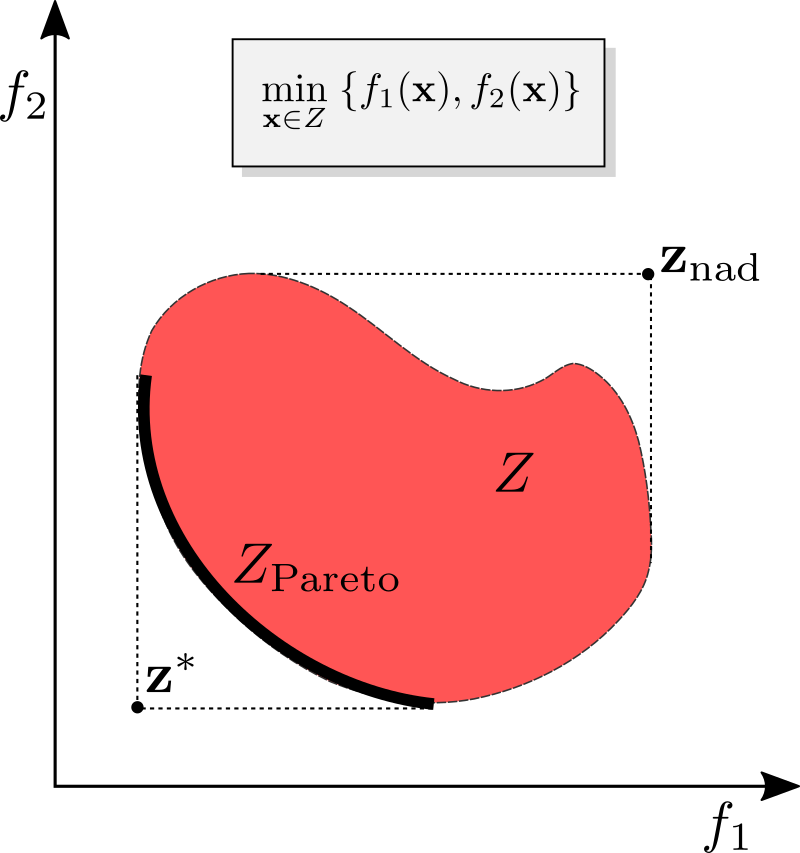
\includegraphics[width=8cm]{contents/moo_concepts.png}
    \caption{\emph{The central concepts of multi-objective optimization conceptualized graphically for a problem with two objectives. The objective function value vector set $Z$
    (filled area), the
    Pareto solution set $Z_{\text{Pareto}}$ (the thick line segment), the ideal point $\mathbf{z}^*$, and the nadir point $\mathbf{z}_{\text{nad}}$, are pictured.
    }}
    \label{fig:moo_concepts}
\end{figure}

The central concepts presented in this section have been conceptualized visually in figure \ref{fig:moo_concepts}
for a multi-objective optimization problem with two objective functions, that are to be minimized.
The Pareto optimal set in figure \ref{fig:moo_concepts} is convex, which is evident in the graphical continuity
of the line segments representing the Pareto optimal set. A non-convex Pareto optimal set would be graphically discontinuous.

\section{Solving multi-objective optimization problems}
\label{mcdmsolve}
{\color{red}
Solving multi-objective optimization problems, what is scalarization and what are ASFs.
}
Multi-objective optimization problems are not straight forward to solve, because the solution is not unambiguous. Without
any kind of preference information, it is impossible in a Pareto optimal set to say that one solution is better than the other.
The number of possible Pareto optimal solution can also be very large, even uncountable, which poses its' own challenges: How many
Pareto optimal solutions should be solved for? Should the Pareto optimal set be evenly distributed? Is some region of the Pareto optimal
set more preferable than others? This section presents methods for solving multi-objective optimization methods by means of scalarization.
A brief overview of other existing methods is also given, and references to the methods described are provided.

\subsection{A word on solving single-objective optimization problems}
\label{solvingsingle}
The crucial methods for solving multi-objective optimization problems, relevant to this thesis, boil down to solving
single-objective optimization problem(s), that capture some sort of given preference, which is defined in section \ref{mcdmdm},
and produce a
solution to the original multi-objective optimization problem, which in turn, reflects the given preference. That is why this chapter
starts with a brief discussion about how to solve single-objective optimization problems.

To solve the single-objective optimization problem, it is necessary to find a solution
$\mathbf{x} \in X$ that minimizes \eqref{eq:singleobjectiveproblem}, or maximizes \eqref{eq:minussingleobjectiveproblem}. 
Various methods exist in literature to solve for $\mathbf{x}$.
Examples of typical, and straightforward, methods are the simplex method,
and Newton's method, which are both -- and accompanied by many more similar methods --
presented in \cite[chapter 9 and 10]{williampress2007}, all paired by blueprints for implementing them in software code.

However, relevant to this thesis, two methods emerge: sequential least squares programming (SLSQP) \cite[chapter 10]{jorgenocedal2006},
and Coin-or branch and cut (CBC) \cite{zenodo2018}. SLSQP is very versatile: it is able to solve non-linear constrained single-objective 
optimization problems. When training belief rule-based system, as discussed in section \ref{training}, the emerging problem to be
solved is a single-objective constrained non-linear optimization problem, which SLSQP is able to solve.

CBC is suitable for solving mixed integer problems: problems were the decision vector variables have real and integer valued
elements. Therefore, CBC is suitable for solving the emerging achievement scalariztion functions, when solving for the Pareto optimal set
in the Finnish forestation case study discussed in section \ref{finnishforestation}.

This subsection will not delve further into the details of each method. For the rest of this section, it is assumed that a method
for solving constrained non-linear single-objective optimization problems exists.

\subsection{Scalarization}
The vector valued objective function present in multi-objective optimization problems \ref{eq:multiobjectiveproblem}, can be transformed
into a vector valued function using some scalarizing function transformation:

\begin{equation}
    \label{eq:funstransform}
    \mathbf{f}: \mathbb{R}^n \to \mathbb{R}^M \;\xrightarrow{{\text{scalarization}}}\; f: \mathbb{R}^n \to \mathbb{R}.
\end{equation}

Therefore, the multi-objective optimization problem is reduced to a single-objective optimization problem, which can be solved using
methods discussed in \ref{solvingsingle}.

As an example, the weighting method transforms the multi-objective optimization problem \ref{eq:multiobjectiveproblem}
into the single-objective problem

\begin{equation}
    \label{eq:weighting}
    \max_{\mathbf{x} \in X} \sum_{i=1}^{M} w_i f_i(\mathbf{x}) \; ,\quad\text{where}\;\sum_{i=1}^{M}w_i = 1\;\text{and}\;w_i \ge 0\;\forall i\in [1, M].
\end{equation}

In problem \eqref{eq:weighting}, $w_i$ are weights associated to the $i$th objective function in the original multi-objective optimization problem. It is proven in
\cite[chapter 3.1]{Miettinen1998}, that when the solution to \ref{eq:weighting} is found, it is Pareto optimal, if the weights $w_i$ are all positive, and the solution
found is unique.

The weighting method is able to produce different Pareto solutions with a different choice of weights. However, there are limitations to the extent of
its' ability to produce Pareto optimal solutions. If the underlying Pareto optimal set is non-convex, the weighting method cannot find all the
solutions\cite[chapter 3.1]{Miettinen1998}. See also \cite{Das1997} for further criticism on generating Pareto optimal solution sets using weighted
sums.

Therefore, the main merit of the weighting method is in its' simplicity, and ease of implementation.
An overview
of other existing scalarization functions can be found in \cite{Coello2017}.

\subsection{Achievement scalarizing functions}
\label{asf}
Achievement scalarizing functions are a set of scalarization function to scalarize multi-objective optimization problems. Achievement scalarizing function are
scalar valued functions of the form

\begin{equation}
    \label{eq:asf}
    s_{\mathbf{\bar{z}}}: \mathbb{R}^M \to \mathbb{R}:\;s_{\mathbf{\bar{z}}}(\mathbf{z}) = s_{\mathbf{\bar{z}}}(\mathbf{f(\mathbf{x}})),
\end{equation}

where $\mathbf{\bar{z}} \in \mathbb{R}^M$ is a reference point, and $\mathbf{f}$ is the objective function of a multi-objective optimization problem
\ref{eq:multiobjectiveproblem}. Using an achievement scalarizing function, an achievement problem

\begin{equation}
    \label{eq:asfproblem}
    \min_{\mathbf{z}\in Z}\; s_{\mathbf{\bar{z}}}(\mathbf{z})
\end{equation}

can be formulated. It is proven in \cite[chapter 3.5]{Miettinen1998}, that when \eqref{eq:asf} is increasing, and the solution to the achievement problem
is unique, then the solution is Pareto optimal. For solving \eqref{eq:asfproblem}, it is required to find an objective vector $\mathbf{z}$, which minimizes
\eqref{eq:asfproblem}. Methods discussed in \ref{mcdmsolve}, are suitable for solving achievement problems as well.

In the case study discussed in \ref{casestudy}, a Pareto optimal set is generated using an achievement scalarizing function, which will be
referred to as the guess function, used in the
GUESS method \cite{Buchanan1997}

\begin{equation}
    \label{eq:guessasf}
    s_\mathbf{\bar{z}}(\mathbf{z}) = \max_{i \in [1, M]}
    \left[ \frac{z_i - z_i^{\text{nad}}}
    {z_i^{\text{nad}} - \bar{z}_i}
    \right],
\end{equation}

where $z_i$ and $\bar{z}_i$ are the components of the objective value vector $\mathbf{z}$ and $\mathbf{\bar{z}}$ respectively. Intuitively,
the guess function, when minimized, results in a Pareto optimal objective value vector $\mathbf{z}$, which has components $z_i$ that have the minimized maximum
deviation, in each component, compared to the nadir point, and which resides on a line segment connecting the reference point and the nadir point.
This is a very straight forward way of calculating a Pareto optimal solution, with minimal assumptions made. Only the nadir point of the original
multi-objective optimization problem is required, and the reference point chosen must be smaller\footnote{Or bigger, if maximization is desired in the
underlying multi-objective optimization problem.}
in every component compared to the nadir point.
How to generate nadir points will be discussed later. In
\cite[chapter 5.7]{Miettinen1998}, it is shown that any Pareto optimal solution can be found when using the guess function.

The guess function can be used to generate a representation of a Pareto optimal set, for a multi-objective optimization problem, by
generating a set of reference points, and solving the achievement scalarizing problem \eqref{eq:asfproblem} using the guess function.
This method of solving for the Pareto optimal set is somewhat similar to the the normal-boundary intersection method \cite{Das1998},
where a set of reference points is also generated, but the analytical form of the objective functions must be
available\footnote{The problem must be either formulated mathematically, or some  surrogate model modelling the
objective functions must be available.}, which is not the case when using an achievement scalarization function.
The guess function has also the advantage to
not suffer from the same limitations as the weighted method \eqref{eq:weighting} mentioned earlier.

Examples of other available achievement scalarization functions, and their comparisons, can be found in \cite{Miettinen2002}.

\section{The decision maker and preference}
\label{mcdmdm}
{\color{red}
What is meant by a decision maker and what is their role. Preference as a concept and utility functions as a model of that concept.
}

So far, only the optimization aspect of multiple criteria decision making has been discussed. This section presents the concept of a decision maker,
and preference, which are in a central role in multiple criteria decision making.

\subsection{The decision maker}
In the context on multiple criteria decision making, the decision maker is usually a human, who is an expert in some field.
The decision maker can be singular, or it can be a group of decision makers. When a group of decision makers is in question,
it is referred to as group decision making. The decision maker can also be artificial, for example an expert system. However,
in the scope of this thesis, only the case of a decision maker, consisting of a single human expert, is of concern.

The role of the decision maker is that of providing preference information, which is not evident
from the general formulation of a multi-objective optimization problems. Preference information can be given by the decision maker
in different forms, and at different times, when solving a multi-objective optimization problem.

When preference is given before a multi-objective optimization problem is solved, preference is said to be given a priori. When preference is
given after a Pareto optimal set has been solved for a multi-objective optimization problem, preference is said to be given a posteriori.
Preference can also be given interactively, which means it is given during the process of solving a multi-objective optimization problem.
Different methods for solving multi-objective optimization problems are usually classified using these three terms: a priori methods,
a posteriori methods, and interactive methods.


\section{Interactivity}
\label{mcdminter}
{\color{red}
Interactivity in MCDM problems, what is meant and why.
}